\documentclass[../main.tex]{subfiles}

\begin{document}

\chapter{Vectors and Vector Spaces}

If you have backgrounds on physics or computer science, you are
probably familiar with what vectors are. In physics classes,
we learn that vectors are quantities with magnitude and direction.
In computer science, vectors are introduced as lists or arrays of
data. Both definitions capture different aspects of what vectors
are. Throughout the notes, we will implement both understandings.
In this note, we will discuss fundamental terms for vectors and
vector spaces before implementing matrices in vector spaces.
Also, most of the heavy abstractions are done is modern algebra,
so it will be an introduction.

\section{Basic Terms and Notations}

First, let's get started by building from definitions.

\begin{definition}
\textbf{Vectors} are mathematical objects, or quantities, with
direction and magnitude. \textbf{Scalars} are real or complex
numbers that does not have direction.
\end{definition}

Vector is a more general term that includes different objects like
matrices and polynomials. Before we discuss about vector spaces,
let's clarify common notations.

\begin{definition}
$\mathbb{R}$ and $\mathbb{C}$ denotes the set of real and complex
numbers respectively. Epsilon symbols $\in$ and $\notin$ is used to
denote whether an element is in the set or not.
\end{definition}

Examples of using such notations would be $\pi \in \mathbb{C}$
and $i \notin \mathbb{R}$.

\begin{definition}
A \textbf{vector space} is a set of vectors $\mathbb{V}$ and scalars
with vector addition and scalar multiplication that adheres to the
following ten properties, or \textbf{axioms for a vector space}.
\begin{enumerate}[noitemsep]
\item[]
\item[] Vector Addition
\item[A1.] \textbf{Closure:}
$\forall \, u, v \in \mathbb{V}$, $u \oplus v \in \mathbb{V}$.
\item[A2.] \textbf{Commutativity:}
$\forall \, u, v \in \mathbb{V}$, $u \oplus v = v \oplus u$.
\item[A3.] \textbf{Associativity:}
$\forall \, u, v, w \in \mathbb{V}$, $u \oplus (v \oplus w) =
(u \oplus v) \oplus w$.
\item[A4.] \textbf{Additive Identity Element:}
$\exists \, 0 \in \mathbb{V}$ such that $\forall \, u \in \mathbb{V},
u \oplus 0 = u$, also known as the \textbf{zero vector}.
\item[A5.] \textbf{Additive Inverses:}
$\forall \, u \in \mathbb{V}, \exists \, -u \in \mathbb{V}$ such that
$u \oplus (-u) = 0$.
\item[]
\item[] Scalar Multiplication
\item[S1.] \textbf{Closure:}
$\forall \, u \in \mathbb{V}$ and scalars $\alpha$, $\alpha \odot
u \in \mathbb{V}$.
\item[S2.] \textbf{Associativity:}
$\forall \, u \in \mathbb{V}$ and scalars $\alpha, \beta$,
$\alpha \odot (\beta \odot u) = (\alpha \cdot \beta) \odot u$.
\item[S3.] \textbf{Identity Element:}
$\forall \, u \in \mathbb{V}$, $1 \odot u = u$.
\item[S4.] \textbf{Distributivity I:}
$\forall \, u \in \mathbb{V}$ and scalars $\alpha, \beta$,
$(\alpha + \beta) \odot u = \alpha \odot u \oplus
\beta \odot u$.
\item[S5.] \textbf{Distributivity II:}
$\forall \, u, v \in \mathbb{V}$ and scalars $\alpha$,
$\alpha \odot (u \oplus v) = \alpha \odot u \oplus \alpha \odot v$.
\end{enumerate}
\end{definition}

Side note here is that for this section of the note, we will be using
the binary operation symbols $\oplus$ and $\odot$ to denote vector
addition and scalar multiplication. However, from the next section,
we will be using more standard notations like $v + u$ and $\lambda v$
for vector addition and scalar multiplication. The reason I decided to
use this is because this is the way I first learned and it helped me
to emphasize axioms for vector spaces.

Based on the scalars that we have here, we could indicate vector
spaces with the following terms.

\begin{definition}
If the set of scalars are in $\mathbb{R}$, then the vector space
is known as a \textbf{vector space over $\mathbb{R}$}, or a
\textbf{real vector space}. Similarly, if the scalars are in
$\mathbb{C}$, then the vector space is denoted as a
\textbf{vector space over $\mathbb{C}$}, or a \textbf{complex vector
space}.
\end{definition}

One thing note is that there is a concept called \textbf{scalar
fields}; however, we will not go too deep into such fields.
Before we move on to different concepts in vector spaces, I wanted
to discuss about tuples and dimensions.

\begin{definition}
An \textbf{$n$-tuple} is an ordered array, or list, of $n$ real
numbers. For an $n$-tuple, its dimension is said to be $n$-dimensional
and the set of such real tuples is \textbf{$n$-space}, denoted as
$\mathbb{R}^n$.
\end{definition}

For instance, the following $4$-tuple is in $4$-space.
\[
\begin{bmatrix}
    1 & 2 & 3 & 4
\end{bmatrix}
\in
\mathbb{R}^4
\]
With tuples in mind, let's take a look at how we can represent
$2$-tuples, $3$-tuples, and vectors in $\mathbb{R}^2$ and
$\mathbb{R}^3$. The vector space $\mathbb{R}^2$ can simply be
conceived as $2$-dimensional space, or plane. Also, in linear
algebra, we generally don't move the tail of a vector from the origin
as we do in introductory physics classes.

\begin{figure}[H]
\centering
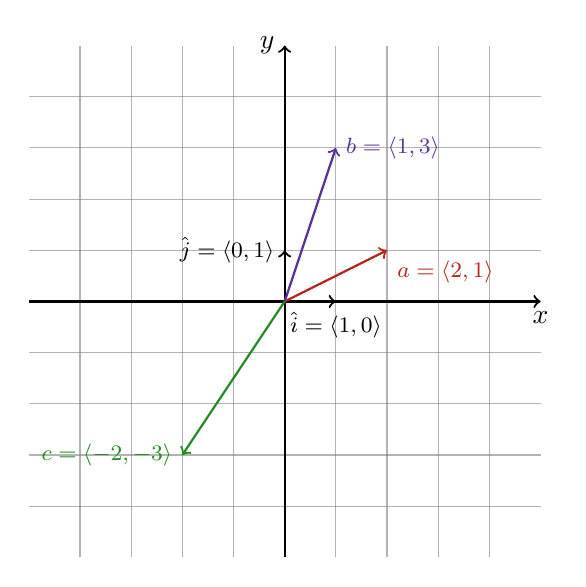
\begin{tikzpicture}[
        vector/.style={->, thick},
        scale=0.65
    ]

    \foreach \i in {-4, -3, ..., 4} {
        \draw[gray, thin, opacity=0.6] (\i, -5) -- (\i, 5);
        \draw[gray, thin, opacity=0.6] (-5, \i) -- (5, \i);
    }
    \draw[vector, black] (-5, 0) -- (5, 0) node[below] {$x$};
    \draw[vector, black] (0, -5) -- (0, 5) node[left] {$y$};

    \draw[vector] (0, 0) -- (1, 0) node[below]
        {\footnotesize $\hat{i} = \langle 1, 0 \rangle$};
    \draw[vector] (0, 0) -- (0, 1) node[left]
        {\footnotesize $\hat{j} = \langle 0, 1 \rangle$};

    \draw[vector, BrickRed] (0, 0) -- (2, 1)
        node[below right, BrickRed]
            {\footnotesize $a = \langle 2, 1 \rangle$};
    \draw[vector, RoyalPurple] (0, 0) -- (1, 3)
        node[right, RoyalPurple]
            {\footnotesize $b = \langle 1, 3 \rangle$};
    \draw[vector, ForestGreen] (0, 0) -- (-2, -3)
        node[left, ForestGreen]
            {\footnotesize $c = \langle -2, -3 \rangle$};
\end{tikzpicture}
\end{figure}

From the graph above, there are two vectors $\hat{i}$ and $\hat{j}$.
They are called ``$i$ hat'' and ``$j$ hat'' respectively.

\begin{definition}
\textbf{Unit Vectors} are vectors with magnitude $1$ that are used to
specify direction.
\end{definition}

Here, $\hat{i}$ and $\hat{j}$ denote the unit vectors, and they are
the standard symbol. If you wondered if unit vectors are used to
construct vectors, you are right! In our examples above, we can
write each vectors as the following.
\begin{align*}
    a &= \langle 2, 1 \rangle = 2 \hat{i} + \hat{j} \\
    b &= \langle 1, 3 \rangle = 1 \hat{i} + 3 \hat{j} \\
    c &= \langle -2, -3 \rangle = -2 \hat{i} - 3 \hat{j}
\end{align*}
Now, let's take a look at vector space $\mathbb{R}^3$. There are
two ways of graphing $3$-dimensional space: right-handed system
and left-handed system. However, we will be using right-hand system
throughout the notes.

\begin{figure}[H]
\centering
\tdplotsetmaincoords{80}{100}
\begin{tikzpicture}[
        tdplot_main_coords,
        axis/.style={->, thick},
        vector/.style={->, very thick},
        scale=0.5
    ]

    \foreach \x in {0,1,...,9}
        \foreach \y in {0,1,...,9} {
			\draw[gray,very thin]
                (\x,0,0) -- (\x,9.5,0);
			\draw[gray,very thin] (0,\y,0) -- (9.5,\y,0);
		}
    \foreach \y in {0,1,...,9}
        \foreach \z in {0,1,...,9} {
			\draw[gray,very thin]
                (0,\y,0) -- (0,\y,9.5);
			\draw[gray,very thin] (0,0,\z) -- (0,9.5,\z);
		}
    \foreach \z in {0,1,...,9}
        \foreach \x in {0,1,...,9} {
			\draw[gray,very thin]
                (0,0,\z) -- (9.5,0,\z);
			\draw[gray,very thin] (\x,0,0) -- (\x,0,9.5);
		}

	\draw[axis] (-2,0,0) -- (10,0,0) node[left] {$x$};
	\draw[axis] (0,-1,0) -- (0,10,0) node[right] {$y$};
	\draw[axis] (0,0,-1) -- (0,0,10) node[left] {$z$};

    \draw[vector] (0, 0, 0) -- (1, 0, 0) node[left]
        {\footnotesize $\hat{i} = \langle 1, 0, 0 \rangle$};
    \draw[vector] (0, 0, 0) -- (0, 1, 0) node[right]
        {\footnotesize $\hat{j} = \langle 0, 1, 0 \rangle$};
    \draw[vector] (0, 0, 0) -- (0, 0, 1) node[above]
        {\footnotesize $\hat{k} = \langle 0, 0, 1 \rangle$};

    \draw[vector, BrickRed] (0, 0, 0) -- (1, 2, 4)
        node[above, BrickRed]
            {\footnotesize $a = \langle 1, 2, 4 \rangle$};
    \draw[vector, RoyalPurple] (0, 0, 0) -- (5, 8, 3)
        node[right, RoyalPurple]
            {\footnotesize $b = \langle 5, 8, 3 \rangle$};
\end{tikzpicture}
\end{figure}

Here, $\hat{i}$, $\hat{j}$, and $\hat{k}$ are the unit vectors.
Going back to the definition of vector spaces, we can write the
following equations for $u = \langle x_1, y_1, z_1 \rangle,
v = \langle x_2, y_2, z_2 \rangle \in \mathbb{R}^3$ and $\alpha
\in \mathbb{R}$.
\begin{align*}
    u \oplus v
    &= \langle x_1, y_1, z_1 \rangle + \langle x_2, y_2, z_2 \rangle
    = \langle x_1 + x_2, y_1 + y_2, z_1 + z_2 \rangle \\
    \alpha \odot u
    &= \alpha \odot \langle x_1, y_1, z_1 \rangle
    = \langle \alpha x_1, \alpha y_1, \alpha z_1 \rangle
\end{align*}
Now that we saw some geometrical interpretation of vector spaces,
let's discuss more information with some problems.

\section{Fundamental Properties}

Let's first start by solving some problems.

\begin{problem}
Identify if the set $\mathbb{S} = \{ (x, y) \in \mathbb{R}^2 \mid
x + y = 5 \}$ is a vector space.
\end{problem}
\begin{solution}
We could see if the set satisfies all axioms for a vector space.
However, just by looking at the condition $x + y = 5$, we know that
there cannot exist a zero vector since $0 + 0 \neq 5$. Because the
set violates A4, the set is not a vector space.
\end{solution}

\begin{problem}
Identify if the set $\mathbb{S} = \{ \langle x, y \rangle \in
\mathbb{R}^2 \mid x + y = 0 \}$ is a vector space.
\end{problem}
\begin{solution}
Unlike the previous problem, we know that there exists a zero
vector. For this one, let's go through each axioms. Let $u =
\langle x_1, -x_1 \rangle$ and $v = \langle x_2, -x_2 \rangle$.
Notice that $u \oplus v = \langle x_1 + x_2, -x_1 - x_2 \rangle
\in \mathbb{R}^2$ and satisfies the condition $x_1 + x_2 + (-x_1
-x_2) = 0$. Therefore, A1 is satisfied. Moreover, consider the
following equations for A2 and A3 where $w = \langle x_3, -x_3
\rangle$.
\begin{align*}
    u \oplus v
    &= \langle x_1, -x_1 \rangle + \langle x_2, -x_2 \rangle
    = \langle x_1 + x_2, -x_1 - x_2 \rangle \\
    &= \langle x_2 + x_1, -x_2 - x_1 \rangle
    = \langle x_2, -x_2 \rangle + \langle x_1, -x_1 \rangle \\
    &= v \oplus u \\
    u \oplus (v \oplus w)
    &= \langle x_1, -x_1 \rangle + \left(
        \langle x_2, -x_2 \rangle + \langle x_3, -x_3 \rangle
    \right) \\
    &= \langle x_1, -x_1 \rangle +
        \langle x_2 + x_3, -x_2 - x_3 \rangle \\
    &= \langle x_1 + x_2 + x_3, -x_1 - x_2 - x_3 \rangle \\
    &= \langle x_1 + x_2, -x_1 - x_2 \rangle +
        \langle x_3, -x_3 \rangle \\
    &= (u \oplus v) \oplus w
\end{align*}
Therefore, A2 and A3 are satisfied. Furthermore, notice that
$\langle 0, 0 \rangle \in \mathbb{R}^2$ and $0 + 0 = 0$, satisfying
A4. Lastly for vector addition A5 holds as $\langle -x, x \rangle$
is the additive inverse of $\langle x, -x \rangle$ that satisfies
the provided conditions. Thus, all axioms for vector addition are met.

Continuing with scalar multiplication, notice that S1 and S3 satisfies
as $\langle x, y \rangle \in \mathbb{R}^2$ and $1 \odot \langle x, y
\rangle = \langle x, y \rangle$. Moreover, consider the following
equations for $\alpha, \beta \in \mathbb{R}$.
\begin{align*}
    \alpha \odot (\beta \odot u)
    &= \alpha \odot \langle \beta x_1, -\beta x_1 \rangle
    = \langle \alpha\beta x_1, -\alpha\beta x_1 \rangle
    = \alpha\beta \odot \langle x_1, -x_1 \rangle \\
    &= (\alpha\beta) \odot u \\
    (\alpha + \beta) \odot u
    &= \langle (\alpha + \beta) x_1, -(\alpha + \beta) x_1 \rangle
    = \langle \alpha x_1 + \beta x_1,
        -\alpha x_1 - \beta x_1 \rangle \\
    &= \langle \alpha x_1, -\alpha x_1 \rangle +
        \langle \beta x_1, -\beta x_1 \rangle \\
    &= \alpha \langle x_1, -x_1 \rangle +
        \beta \langle x_1, -x_1 \rangle \\
    &= \alpha \odot u \oplus \beta \odot u \\
    \alpha \odot (u \oplus v)
    &= \alpha \langle x_1 + x_2, -x_1 - x_2 \rangle
    = \langle \alpha x_1 + \alpha x_2,
        -\alpha x_1 - \alpha x_2 \rangle \\
    &= \langle \alpha x_1, -\alpha x_1 \rangle +
        \langle \alpha x_2, -\alpha x_2 \rangle \\
    &= \alpha \langle x_1, -x_1 \rangle +
        \alpha \langle x_2, -x_2 \rangle \\
    &= \alpha \odot u \oplus \alpha \odot v
\end{align*}
Thus, S2, S4, and S5 are all satisfied. Because all ten axioms for
a vector space are met, the set $\mathbb{S} = \{ \langle x, y \rangle
\in \mathbb{R}^2 \mid x + y = 0 \}$ is a vector space.
\end{solution}

\begin{problem}
Consider vectors in the form $\langle x, y, z \rangle$ where the
vector addition is defined as $\langle x, y, z \rangle \oplus
\langle x', y', z' \rangle = \langle x + x', y + y', z + z' \rangle$
and scalar multiplication as $\alpha \langle x, y, z \rangle =
\langle x^\alpha, y^\alpha, z^\alpha \rangle$. Identify if the vectors
form a vector space.
\end{problem}
\begin{solution}
First, notice that the vector addition adheres to the standard vector
addition. Therefore, we only have to look at scalar multiplication
if any axioms are violated. From glance, S1, S2, and S3 appears to
be satisfied. Therefore, let's take a look at S4.
\[
(\alpha + \beta) \odot u
= \left(
    x^{\alpha + \beta}, y^{\alpha + \beta}, z^{\alpha + \beta}
\right)
\]
Notice that in general, $x^{\alpha + \beta} \neq x^\alpha + x^\beta$.
Therefore, the set of vectors do not form a vector space.
\end{solution}

Just as we have vector spaces $\mathbb{R}^n$, we could also define
spaces depending on the objects.

\begin{definition}
The symbol $\mathbb{P}^n$ denotes the vector space composed of
polynomials of degree at most $n$ and adheres to the ten properties.
$\mathbb{M}_{m \times n}$ represents the vector space with matrices
of order $m \times n$ that adheres to the ten properties.
\end{definition}

Therefore, we can say that $\mathbb{R}^n$ is more or less same as
$\mathbb{M}_{1 \times n}$. With the understandings above, we can
derive some important theorems. Although most of them are intuitive,
its always nice to formally prove them so let's do that now.

\begin{theorem}{Uniqueness of the Zero Vector}
For all vector spaces, zero vector, or the additive identity element,
is unique.
\end{theorem}
\begin{proof}
For the sake of contradiction, let $0_1, 0_2 \in V$ be distinct
additive identity element for a vector space $V$. By definition,
the following equations hold.
\begin{align*}
    0_1 \oplus 0_2 &= 0_1 \\
    0_1 \oplus 0_2 &= 0_2 \\
    \therefore 0_1 \oplus 0_2 &= 0_1 = 0_2
\end{align*}
Because $0_1 = 0_2$ is contradictory from the fact that $0_1$ and
$0_2$ are distinct, the initial assumption that there exists distinct
additive identity element in a vector space is false.
\end{proof}

Continuing from the uniqueness of the zero vector in a vector space,
we can assert the following theorem.

\begin{theorem}{Uniqueness of Additive Inverse}
For all $u \in V$ for any vector space $V$, $v \in V$ such that
$u \oplus v = 0$ is unique.
\end{theorem}
\begin{proof}
For the sake of contradiction, assume $v, w \in V$ are distinct
additive inverses of $u$. By definition and properties of vector
spaces, the following equations hold.
\[
v
= v \oplus 0
= v \oplus (u \oplus w)
= (v \oplus u) \oplus w
= 0 \oplus w
= w
\]
Because $v = w$ contradicts from the definition that $v$ and $w$
are unique, the initial assumption that there exists more than one
additive inverse of a vector in vector spaces is false.
\end{proof}

Just as $x = 0$ if $x + x = x$, we could do similar things in vector
spaces.

\begin{theorem}{Property of Zero Vectors I}
For all $v \in V$ and any vector space $V$, $v \oplus v = v$ if and
only if $v = 0$.
\end{theorem}
\begin{proof}
First, the first half of the statement can be proven. Consider the
following equations.
\begin{align*}
    (v \oplus v) \oplus (-v)
    &= v \oplus (-v) = 0 \\
    &= v \oplus (v \oplus (-v)) = v \oplus 0 = v
\end{align*}
Therefore, if $v \oplus v = v$, then $v = 0$. Moreover, if $v = 0$,
then $v \oplus v = 0 \oplus 0 = 0$. Therefore, the premise holds.
\end{proof}

Now let's take a look at theorems for scalar multiplications.

\begin{theorem}{Properties of Scalar Multiplications}
The following properties hold for all vector space $V$ over
$\mathbb{F}$, $u, \mathbf{0} \in V$, and any scalars $\alpha$.
\begin{enumerate}[noitemsep]
\item $0 \odot u = \mathbf{0}$
\item $\alpha \odot \mathbf{0} = \mathbf{0}$.
\item $(-1) \odot u = -u$
\item $u = -(-u)$
\item $\alpha \odot u = \mathbf{0}$ if and only if $\alpha = 0$ or
$u = \mathbf{0}$.
\end{enumerate}
\end{theorem}

Let's start with the first proof.

\begin{proof}
Consider the following equation.
\[
0 \odot u
= (0 + 0) \odot u
= 0 \odot u \oplus 0 \odot u
\]
By Theorem \ref{theo:Property of Zero Vectors I}, $0 \odot u =
\mathbf{0}$.
\end{proof}

Below is the proof for the second property.

\begin{proof}
Consider the following equation.
\[
\alpha \odot \mathbf{0}
= \alpha \odot (\mathbf{0} \oplus \mathbf{0})
= \alpha \odot \mathbf{0} \oplus \alpha \odot \mathbf{0}
\]
By Theorem \ref{theo:Property of Zero Vectors I}, $\alpha \odot
\mathbf{0} = \mathbf{0}$
\end{proof}

Continuing, here's the proof for the third one.

\begin{proof}
By the properties of vector spaces, $\mathbf{0} = 0 \odot u =
(1 - 1) \odot u = 1 \odot u \oplus (-1) \odot u = u \oplus (-1)
\odot u $. Because $(-1) \odot u$ is the additive inverse of $u$,
$(-1) \odot u = -u$.
\end{proof}

Below is the proof for the fourth one.

\begin{proof}
Notice that $-(-u)$ is the additive inverse of $-u$. However, by
definition, $u$ is the additive inverse of $-u$. By Theorem
\ref{theo:Uniqueness of Additive Inverse}, $u = -(-u)$.
\end{proof}

Finally, let's prove the last property.

\begin{proof}
It suffices to show the latter half of the statement as the first
half is shown by the first two properties. Consider the following
equations for $\alpha \neq 0$.
\begin{align*}
    \frac{1}{\alpha} \odot (\alpha \odot u)
    &= \frac{1}{\alpha} \odot \mathbf{0}
    = \mathbf{0} \\
    &= \left( \frac{1}{\alpha} \cdot \alpha \right) \odot u
    = 1 \odot u
    = u
\end{align*}
Therefore, if $\alpha \neq 0$, then $u = \mathbf{0}$. Similarly,
if $u \neq \mathbf{0}$, then $\alpha = 0$ as the product of nonzero
numbers is a nonzero number.
\end{proof}

We have covered the fundamental concepts and properties in vector
spaces. Before we move on with the next topic in vector spaces,
I wanted to discuss briefly on dot product as it will frequently
appear when you deal with vectors.

\begin{definition}
\textbf{Dot product} is an algebraic operation defined as the
following for vectors $a = [ a_1, \ldots, a_n]$ and $b =
[ b_1, \ldots, b_n]$
\[
a \cdot b
= \sum_{k = 1}^n a_k b_k
\]
\end{definition}

Here notice that the number of elements of the vectors in dot product
must be equal for the product to be defined. Below are some examples
of dot products.
\begin{align*}
\begin{bmatrix}
    1 \\
    2 \\
    3
\end{bmatrix}
\cdot
\begin{bmatrix}
    -1 \\
    -2 \\
    -3
\end{bmatrix}
&= 1(-1) + 2(-2) + 3(-3)
= -14 \\
\begin{bmatrix}
    0 & 1 & 2
\end{bmatrix}
\cdot
\begin{bmatrix}
    0 & 1 & 0
\end{bmatrix}
&= 0 \cdot 0 + 1 \cdot 1 + 2 \cdot 0
= 1
\end{align*}

Note that this is very different from the matrix multiplication
that we will discuss in the next note and we must write the
notation $\cdot$ to ensure that we are not doing matrix
multiplication. With that in mind, let's continue our discussion
with subspaces.

\section{Subspaces}

In the previous section, we discussed that all ten axioms must be
satisfied for a set to be a vector space. However, testing and
proving that a set satisfies all ten axioms, to be honest, is quite
tedious. Good news is that we only need to prove three conditions to
show that a set is a vector space thanks to \textbf{subspaces}!

\begin{definition}
A \textbf{subspace} of a vector space $V$ is a subset of $V$ that uses
the same definition of vector addition and scalar multiplication from
$V$.
\end{definition}

Now for a set to be a subspace, it must satisfy the following
conditions.

\begin{theorem}{Conditions of a Subspace}
A non-empty subset $S$ of a vector space $V$ is a subspace of $V$ if
and only if the following conditions are satisfied.
\begin{enumerate}[noitemsep]
\item
\textbf{Closure for Addition: }
$\forall u, v \in S, u + v \in S$
\item
\textbf{Closure for Scalar Multiplication: }
$\forall u \in S$ and scalars $\alpha$, $\alpha u \in S$
\end{enumerate}
\end{theorem}
\begin{proof}
Notice that it suffices to show that $S$ is a vector space, or adhere
to the then axioms for a vector space. Moreover, A1 and S1 are assumed
to be true by the initial condition.

By the second condition, $\mathbf{0} = 0 u \in S$ and $-u = (-1) u
\in S$. Therefore, A4 and A5 are satisfied. For A2 and A3, $u, v, w
\in V$ is true for $u, v, w \in S$ by definition. Moreover, because
$V$ is a vector space, A2 and A3 holds. Similarly, because $V$ is a
vector space that satisies S1, S2, S3, S4, and S5, its subset $S$ also
satisfy the conditions. Therefore, if the two closure conditions are
met and $S$ is a subset of $V$, then $S$ is a subspace of $V$.
\end{proof}

Now the good thing is that subspaces are vector spaces, it suffices
to show that a set is a subspace of a known vector space with the two
conditions shown above to show that it is a vector space. Let's take
a look at an example.

\begin{problem}
Determine whether $S = \{ (x, y, z) \in \mathbb{R}^3 \mid y = 0 \}$
is a vector space.
\end{problem}
\begin{solution}
Notice that $S$ is an non-empty subset of $\mathbb{R}^3$, which is a
known vector space. Therefore, it suffices to show that $u =
(x_1, 0, z_1), v = (x_2, 0, z_2) \in S$ and scalars $\alpha$ satisfy
the closure conditions for addition and scalar multiplication.

Notice that $u + v = (x_1 + x_2, 0, z_1 + z_2) \in S$. Moreover,
$\alpha u = (\alpha x_1, 0, \alpha z_1) \in S$. Therefore, $S$ is a
vector space, more specifically a subset of $\mathbb{R}^3$.
\end{solution}

As you can see from the solution above, subspaces really made our
lives easier. However, to make it even better, we can boil it down
to a single condition.

\begin{corollary}{The Condition for a Subspace}
For scalars $\alpha$ and $\beta$ and $u, v \in S$ where $S$ is a
non-empty subset of a vector space $V$ that has the same operations
for vector addition and scalar multiplication, $S$ is a subspace if
and only if the following equation is satisfied.
\[
\alpha u + \beta v \in S
\]
\end{corollary}
\begin{proof}
First and foremost, the first half of the statement can be proven.
If $\alpha u + \beta v \in S$, then $u + v \in S$ where $\alpha =
\beta = 1$ since $\alpha$ and $\beta$ are all scalars. Similarly,
$\alpha u + \beta v \in S$ implies that $\alpha u \in S$ where
$\beta = 0$. By Theorem \ref{theo:Conditions of a Subspace}, $S$ is a
subspace of $V$.

Continuing with the second half of the statement, if $S$ is a subset
of $V$, then $\alpha u, \beta v \in S$. Therefore, $\alpha u +
\beta v \in S$, proving the corollary.
\end{proof}

More examples on this can be found in the practice problems below.
Now let's get into the topics of \textbf{linear combination} and the
\textbf{span} of a set.

\subsection{Linear Combinations and Span}

As always, let's start with definitions.

\begin{definition}
For scalars $\alpha_i$ and $v_i$ in a vector space $V$, the vector
$u$ defined as the following is a \textbf{linear combination of the
vectors} $v_i$.
\[
u = \sum_{k = 1}^n \alpha_k v_k
\]
\end{definition}

For instance, $[1, 2, 3]$ is a linear combination of $[2, -2, 1]$,
$[1, 0, 2]$, and $[1, -1, 1]$ as it can be represented as the
following.
\[
\begin{bmatrix}
    1 & 2 & 3
\end{bmatrix}
=
\begin{bmatrix}
    2 & -2 & 1
\end{bmatrix}
+
3\begin{bmatrix}
    1 & 0 & 2
\end{bmatrix}
-
4\begin{bmatrix}
    1 & -1 & 1
\end{bmatrix}
\]
Now we have a special term for the collection of such vectors.

\begin{definition}
The \textbf{span of the set of vectors} $\{ v_1, \ldots v_n \}$ is
the set of all possible linear combinations of the vectors.
\[
\Span\{v_1, \ldots, v_n\}
= \left\{
    \sum_{k = 1}^n \alpha_k v_k \; \middle|\; \alpha_k \in \mathbb{R}
\right\}
\]
\end{definition}

With the definition, we could notice an important theorem.

\begin{theorem}{Span and Subspace I}
For a vector space $V$ and its subset $S = \{ v_1, \ldots, v_n \}$,
$\Span(S)$ is a subspace of $V$.
\end{theorem}
\begin{proof}
First and foremost, notice that $\mathbf{0} \in \Span(S)$ since all
the scalars in linear combination can equal zero. Moreover, let $u =
\sum_{k = 1}^n \alpha_k v_k$ and $v = \sum_{k = 1}^n \alpha_k v_k$ for
any scalars $\alpha_k$ and $\beta_k$. By definition, $\alpha u +
\beta v \in \Span(S)$ is true. Therefore, by Corollary
\ref{cor:The Condition for a Subspace}, $\Span(S)$ is a subspace of
$V$.
\end{proof}

Side note here is that there are spans of infinite sets and they
adhere to the theorem above. Continuing with the definition of the
span of a set and its relation with subspace, we can show the two
following theorems.

\begin{theorem}{Span and Subspace II}
Consider the following statements for a vector space $V$ and its
subspace $W$ and non-empty subset $S$ such that $S \subset W$.
\begin{enumerate}[noitemsep]
\item $\Span(S) \subset W$
\item The intersection of all subspaces containing $S$ is $\Span(S)$.
\end{enumerate}
\end{theorem}

Let's start by proving the first statement.

\begin{proof}
Let $u = \sum_{k = 1}^n \alpha_k v_k \in \Span(S)$. By definition,
$v_k \in W$ for integer $k \in [1, n]$. Moreover, $u \in W$ by
Corollary \ref{cor:The Condition for a Subspace} and $\Span(S)
\subset W$.
\end{proof}

Below is the proof for the second one.

\begin{proof}
First and foremost, notice that by the previous statement, it was
shown that $\Span(S)$ is included in all subspaces that contains $S$.
Let $A$ be the intersection of all subspaces that contain $S$.
Therefore, $\Span(S) \subset A$. Moreover, by Theorem
\ref{theo:Span and Subspace I} $\Span(S)$ is a subspace of $V$ that
contains $S$. Thus, $A \subset \Span(S)$. Because $\Span(S) \subset A$
and $A \subset \Span(S)$, $\Span(S) = A$.
\end{proof}

Next, let's conclude our discussion on linear combination and span
of a set of vectors by proving the following statements.

\begin{theorem}{Four Lemmas on Span of a Set of Vectors}
For a vector space $V$ and its subsets $S, T \subset V$, consider the
following statements.
\begin{enumerate}[noitemsep]
\item If $T \subset S$, then $\Span(T) \subset \Span(S)$.
\item $\Span(\Span(S)) = \Span(S)$.
\item If $T \subset \Span(S)$, then $\Span(T) \subset \Span(S)$.
\item For nonzero vectors $v_1, \ldots, v_n \in V$, scalar
$\lambda \in \mathbb{R}$, and $1 \leq j, k \leq n$ such that $\lambda
\neq 0$ and $j \neq k$, the following equations hold.
\vspace{-0.5\baselineskip}
\begin{align*}
    \Span\{ v_1, \ldots, v_k, \ldots, v_n \}
    &= \Span\{ v_1, \ldots, v_k + \lambda v_j, \ldots, v_n \} \\
    \Span\{ v_1, \ldots, v_k, \ldots, v_n \}
    &= \Span\{ v_1, \ldots, \lambda v_k, \ldots, v_n \}
\end{align*}
\end{enumerate}
\end{theorem}

There's a lot to prove, but let's do them one by one starting with
the first one.

\begin{proof}
Notice that since all $t_k \in T$ satisfy $t_k \in S$, all
$\sum_{k=1}^n c_k t_k \in \Span(T)$ for some appropriate $n$ and
constant $c_k$ also satisfy $\sum_{k=1}^n c_k t_k \in \Span(S)$.
Therefore, $\Span(T) \subset \Span(S)$.
\end{proof}

Below is the proof for the second statement, which is a corollary
of the first statement.

\begin{proof}
First and foremost, notice that $S \subset \Span(S)$. By the first
statement, $\Span(S) \subset \Span(\Span(S))$ holds. Moreover,
notice that because $\Span(S)$ contains all linear combinations of
$S$, making more linear combinations of the linear combinations of
$S$ will not add more elements. Therefore, $\Span(\Span(S)) \subset
\Span(S)$ and $\Span(\Span(S)) = \Span(S)$.
\end{proof}

Continuing, let's prove the third statement.

\begin{proof}
Notice that by the first statement, $\Span(T) \subset
\Span(\Span(S))$. Continuing with the second statement shows that
$\Span(T) \subset \Span(S)$.
\end{proof}

Finally, here is the proof for the last statement.

\begin{proof}
First, it is self-evident that $\Span\{ v_1, \ldots, v_k
+ \lambda v_j, \ldots, v_n \} \subset \Span\{ v_1, \linebreak \ldots,
v_k, \ldots, v_n \}$ since all linear combination of the set of
vectors on the left can be represented as the linear combination of
the set of vectors on the right. Moreover notice that $v_k$ can be
represented as $v_k = (v_k + \lambda v_j) - \lambda v_j$ even if
$k = j$. Therefore, $v_k \in \Span\{ v_1, \ldots, v_k + \lambda v_j,
\ldots, v_n \}$ and $\Span\{ v_1, \ldots, v_k, \ldots, v_n \} \subset
\Span\{ v_1, \ldots, v_k + \lambda v_j, \linebreak \ldots, v_n \}$ by
statement 3. Therefore, the equations in the statement hold.
\end{proof}

With the ideas of linear combinations and the span of a set of vectors
in mind, let's discuss about linear independence.

\subsection{Linear Independence}

One of the most important reason why we use Linear Algebra is due to
efficiency. As you could have guessed, most vector spaces have
infinitely many vectors. Of course, there must be an efficient way
of representing the vector space instead of manually listing.
Determining such representative vectors involve numerous factors,
and that's what we will discuss with linear independence, basis,
and dimension.

\begin{definition}
Consider the linear combination of $V = \{ v_1, \ldots, v_n \}$
in a vector space and scalars $c_1, \ldots, c_n$ that satisfy the
following equation.
\[
\sum_{k = 1}^n c_k v_k = \mathbf{0}
\]
The set of vectors $V$ is \textbf{linearly dependent} if at least
one of the scalars in the equation is nonzero. The set of vectors is
\textbf{linearly independent} all scalars are zero in the equation.
\end{definition}

Let's take a look at a quick example.

\begin{problem}
Determine whether $V = \{ \langle 1, 1 \rangle, \langle 2, 3\rangle
\in \mathbb{R}^2 \}$ is linearly independent.
\end{problem}
\begin{solution}
By definition, for the set to be linearly independent, all scalars
$c_1$ and $c_2$ must be zero for the following equation to hold.
\[
c_1 \langle 1, 1 \rangle + c_2 \langle 2, 3 \rangle
= \langle 0, 0 \rangle
\]
Writing in system of linear equations, the equation above can
be written as the following.
\begin{align*}
    c_1 + 2c_2 &= 0 \\
    c_1 + 3c_2 &= 0
\end{align*}
Solving the equation, $c_1 = c_2 = 0$ and no other set of scalars
can lead to the equation. Therefore, the set of vectors is linearly
independent.
\end{solution}

One interesting observation that we can make is that for $n \in
\mathbb{Z}$, if the set of vectors in $\mathbb{R}^n$ contains more
than $n$ elements, then the set is linearly dependent. We will
discuss more on this later when we discuss matrix and its application
in linear systems, but for such cases, we have more variables than
linear equations, which implies that there exists infinitely many
solutions. Therefore, such set of vectors must be linearly dependent.
Continuing, below is a theorem that we can deduce from the definition.

\begin{theorem}{Finite Set of Vectors and Linear Dependence}
A set with finite number of nonzero vectors is linearly dependent
if and only if a vector in the ordering of the set can be represented
as a linear combination of vectors preceding it.
\end{theorem}
\begin{proof}
First and foremost, the first half of the theorem can be shown.
Consider the set of vectors $\{ v_1, \ldots, v_{j-1}, v_j, \ldots,
v_n \}$. Assume for scalars $c_k$, the following equation is true.
\[
v_j
= \sum_{k = 1}^{j-1} c_k v_k
\]
Therefore, $\mathbf{0} = \sum_{k = 1}^{j-1} c_k v_k - v_j$.
Letting $c_k = 0$ for integer $k \in (j, n]$, the following equation
holds.
\[
\sum_{k = 1}^{j-1} c_k v_k - v_j + \sum_{k = j+1}^{n} c_k v_k
= \mathbf{0}
\]
Because at least scalar is nonzero, the set of vectors $\{ v_1,
\ldots, v_n \}$ is linearly dependent.

Continuing, let the set of vectors $\{ v_1, \ldots, v_n \}$ be
linearly dependent. For the corresponding scalars $c_k$, let
$c_j$ be the last scalar that is nonzero. Thus, the following
equation holds.
\[
\sum_{k = 1}^{j} c_k v_k + \sum_{k = j+1}^{n} 0 v_k
= \mathbf{0}
\]
Rearranging the equation, $v_k = -\sum_{k = 1}^{j-1} \frac{c_k}{v_j}
v_k$, which is a linear combination. Because the converse hold,
the theorem is true.
\end{proof}

From this theorem, we can deduce a corollary.

\begin{corollary}{}
For a vector space $V = \Span(S)$ and linearly dependent set
$S = \{ v_1, \ldots, v_n \} \subset V$, then there exists a set
$T \subset S$ such that $|T| = n - 1$ and $V = \Span(T)$.
\end{corollary}
\begin{proof}
By Theorem \ref{theo:Finite Set of Vectors and Linear Dependence},
there exits element $v_j \in S$ such that $v_j$ is the linear
combination of the previous elements as listed in $S$.

Let $T = \{ v_1, \ldots, v_{j-1}, v_{j+1}, \ldots, v_n \}$.
Consider the following equations for scalars $d_k$ and $c_k$.
\begin{align*}
    V
    &= \sum_{k = 1}^n d_k v_k
    = \sum_{k = 1}^{j-1} d_k v_k + d_j v_j +
        \sum_{k = j+1}^n d_k v_k \\
    &= \sum_{k = 1}^{j-1} d_k v_k +
        d_j \left( \sum_{k = 1}^{j-1} c_k v_k \right) +
        \sum_{k = j+1}^n d_k v_k \\
    &= \sum_{k = 1}^{j-1} (d_j c_k + d_k) v_k +
        \sum_{k = j+1}^n d_k v_k
    = \Span(T)
\end{align*}
Therefore, the corollary holds.
\end{proof}

Continuing from the corollary, the following theorems could be
asserted.

\begin{theorem}{Properties of Linear Independence and Dependence}
Consider the following statements for set $S$.
\begin{enumerate}[noitemsep]
\item
If $S$ contains a zero vector, then it is linearly dependent.
\item
If $|S| = 1$, then it is linearly dependent if and only if its
element is the zero vector.
\item
If $|S| = 2$, then it is linearly dependent if and only if a vector
is a scalar multiple of the other.
\item
If $S$ is linearly dependent, then every set that contains $S$ is
linearly dependent.
\item
If $S$ is linearly independent, all its subset is linearly
independent.
\end{enumerate}
\end{theorem}

There's quite a bit to prove! Let's start with the first one.

\begin{proof}
Let $S = \{ \mathbf{0}, v_1, \ldots, v_n \}$. Notice that
$\alpha(\mathbf{0}) + \sum_{k = 1}^n 0 v_k = \mathbf{0}$ for any
scalar $\alpha$. Therefore, $S$ is linearly dependent.
\end{proof}

Below is the proof for the second one.

\begin{proof}
Let $S = \{ v \}$. Notice that if $v \neq \mathbf{0}$, it is not
possible for a nonzero scalar $\alpha$ to make $\alpha v =
\mathbf{0}$. Therefore, if $|S| = 1$, then $v = \mathbf{0}$.
For the converse, if $v = \mathbf{0}$, then any scalar $\alpha$
will let $\alpha v = \mathbf{0}$. Therefore the statement holds.
\end{proof}

Here is the proof for the third statement.

\begin{proof}
Let $S = \{ v_1, v_2 \}$. First, if $v_2 = \alpha v_1$ for any scalar
$\alpha$, then $\mathbf{0} = \alpha v_1 - \alpha v_1 = \alpha v_1 -
v_2$. Therefore, $S$ is linearly dependent. For the converse,
$c_1 v_1 + c_2 v_2 = 0$ for scalars $c_1$ and $c_2$. Therefore,
assuming that the scalars are nonzero without loss of generality,
$v_2 = -\frac{c_1}{c_2} v_1$. Thus, the statement is true.
\end{proof}

Below is the proof for the fourth one.

\begin{proof}
Let $S = \{ v_1, \ldots, v_n \}$ and $T = \{ u_1, \ldots, u_n,
v_1, \ldots, v_n \}$. By definition, there exists $c_k$ that are
not all zero such that $\sum_{k = 1}^n c_k v_k = \mathbf{0}$.
Because $\sum_{k = 1}^n 0 u_k + \sum_{k = 1}^n c_k v_k = \mathbf{0}$,
$T$ is also linearly dependent.
\end{proof}

Finally, here is the proof for the last statement.

\begin{proof}
Let $T \subset S$ where $S$ is linearly independent. Assume for
the sake of contradiction that there exists a subset $T$ that is
linearly dependent. However, if $T$ is linearly dependent, then
$S$ is linearly dependent by the previous property, which is
a contradiction. Therefore, by contradiction, if $S$ is linearly
independent then all its subsets $T$ is also linearly independent.
\end{proof}

With this, we have concluded our discussion on linear dependence
and independence. Before concluding this note, let's discuss
basis and dimension of a set of vectors.

\subsection{Basis and Dimension}

As always, let's start with definition.

\begin{definition}
For a vector space $V$ and its subset $S$, if $\Span(S) = V$, then
$S$ is a spanning set for $V$.
\end{definition}

When we say aloud, we say that $S$ spans $V$. For instance, the set
$\{ \langle 1, 0 \rangle, \langle 0, 1 \rangle \}$ spans
$\mathbb{R}^2$ since all vectors $\langle a, b \rangle \in
\mathbb{R}^2$ can be represented as the sum $a \langle 1, 0 \rangle
+ b\langle 0, 1 \rangle$.

\begin{definition}
A linearly independent subset that spans $V$ is a \textbf{basis} for
$V$.
\end{definition}

Continuing from the previous example, we can see that $\{ \langle 1, 0
\rangle, \langle 0, 1 \rangle \}$ not only spans $\mathbb{R}^2$,
but is also a basis for $\mathbb{R}^2$ since it is linearly
independent. As you can see, the same will apply if we generalize it
to $\mathbb{R}^n$.

\begin{definition}
The \textbf{standard basis for $\mathbb{R}^n$} is the set $S =
\{ e_1, \ldots e_n \}$ where $e_i$ is the $i\text{th}$ column of
$I_n$.
\end{definition}

We could do the same for polynomials. First, notice that the set
$\{ 1, x, x^2 \}$ spans $\mathbb{P}^2$. Moreover, the set is linearly
independent. Therefore, $\{ 1, x, x^2 \}$ is a basis for
$\mathbb{P}^2$.

\begin{definition}
The \textbf{standard basis for $\mathbb{P}^n$} is the set $S =
\{ 1, x, x^2, \ldots, x^n \}$.
\end{definition}

From the two definitions above, we can notice that there are finite
elements for the two standard basis for $\mathbb{R}^n$ and
$\mathbb{P}^n$. We call such vector spaces
\textbf{finite-dimensional}.

\begin{definition}
A vector spaces with a basis of finite elements is called
\textbf{finite-dimensional}. Whereas, \textbf{infinite dimensional}
vector spaces do not contain a basis with finite elements.
\end{definition}

An example of infinite dimensional vector space would be $\mathbb{P}$
since the basis is required to be an infinite set. However, we will
not be discussing infinite dimensional vector spaces. From the
definitions above, we could establish a theorem.

\begin{theorem}{Basis and Linear Dependence}
For a basis $S$ of a vector space $V$ such that $|S| = n$, any set
in $V$ with more than $n$ elements is linearly dependent.
\end{theorem}
\begin{proof}
Let $S = \{ v_1, \ldots, v_n \}$ and $T = \{ u_1, \ldots, u_m \}$
such that $S, T \in V$ and $m > n$. Notice that because $\Span(S) = V$
and $T \in V$, there exists a set of constants $a_{ij}$ that satisfies
the following equation (note that we will be using this indices in
the next note when we discuss matrices.).
\begin{align*}
    u_1 &= \sum_{j=1}^n a_{1j} v_j \\
    u_2 &= \sum_{j=1}^n a_{2j} v_j \\
    &\quad\vdots \\
    u_m &= \sum_{j=1}^n a_{mj} v_j
\end{align*}
Therefore, it suffices to show that there exists constants $c_1,
\ldots, c_m$ such that not all are zero and that satisfies the
following equation.
\[
\sum_{i=1}^m \sum_{j=1}^n c_i a_{ij} v_j
= \mathbf{0}
\]
Continuing, it suffices to show that the variables $c_i$ and constants
$a_{ij}$ satisfy the following equations where not all $c_i$ are zero.
\begin{align*}
    \sum_{i=1}^m c_i a_{i1} &= 0 \\
    \sum_{i=1}^m c_i a_{i2} &= 0 \\
    &\ \vdots \\
    \sum_{i=1}^m c_i a_{in} &= 0
\end{align*}
Notice that there are $m$ variables and $n$ equations. It is known
that for a linear system of equations, there exists infinite number
of solutions if there are more variables than the equations (don't
worry we will prove this in future notes.). Because $m > n$, there
exists $c_1, \ldots c_m$ that are not all zero and that satisfy the
equations for linear dependence, the theorem holds.
\end{proof}

Continuing, we can derive three corollaries from the theorem.

\begin{corollary}{}
If a basis for the vector space $V$ contains $n$ elements, then any
linearly independent subsets of $V$ contains at most $n$ elements.
\end{corollary}
\begin{proof}
By definition, a basis of a vector space $V$ spans $V$. Because any
linearly dependent subsets of $V$ contains more than $n$ elements
by Theorem \ref{theo:Basis and Linear Dependence}, any linearly
independent subsets of $V$ must not contain more than $n$ elements.
\end{proof}

Below is the second corollary.

\begin{corollary}{}
If $V$ is a finite vector space, every basis of $V$ will contain
the same number of elements.
\end{corollary}
\begin{proof}
Let $S$ and $T$ be bases of $V$ with $p$ and $q$ elements
respectively. By definition, the bases of a vector space is linearly
independent. By the previous corollary, it is evident that $q \leq p$
and $p \leq q$ are true. Therefore, $p = q$ and the corollary holds.
\end{proof}

Now before continuing with our third corollary, let's first define
what the dimension of a vector space is.

\begin{definition}
For a finite dimensional vector space $V$, the number of elements
in any basis of $V$ is called the \textbf{dimension} of $V$,
denoted as $\dim(V)$.
\end{definition}

For instance, recall the standard basis of $\mathbb{R}^n$. From the
number of elements in the basis, we can write that $\dim(\mathbb{R}^n)
= n$. Similarly, we can also notice that $\dim(\mathbb{P}^n) = n + 1$.
Now let's continue with our third corollary.

\begin{corollary}{}
Every set $S$ in an $n$-dimensional vector space such that $|S| =
n + 1$ is linearly dependent.
\end{corollary}
\begin{proof}
By definition, a basis of an $n$-dimensional vector space $V$ contains
$n$ elements. By Theorem \ref{theo:Basis and Linear Dependence}, since
$n + 1 > n$, $S$ must be linearly dependent.
\end{proof}

One fun fact to note is that for the vector space $\{0\}$, we say
$\dim(\{0\}) = 0$ by convention. Moreover, consider the following
theorem.

\begin{theorem}{Unique Linear Combination}
For a basis $S = \{ v_1, \ldots, v_n \}$ of a vector space $V$,
any vector $u \in V$ can be written as a unique linear combination
of $S$.
\end{theorem}
\begin{proof}
For the sake of contradiction, assume that $u$ can be written as
$u = \sum_{k=1}^n c_k v_k = \sum_{k=1}^n d_k v_k$ where $c_k \neq d_k$
for some choice of $k$. Therefore, the following equations can be
obtained.
\begin{align*}
    \sum_{k=1}^n c_k v_k &= \sum_{k=1}^n d_k v_k \\
    \sum_{k=1}^n (c_k - d_k) v_k &= 0
\end{align*}
Note that by definition, $S$ is linearly independent and $c_k - d_k
= 0$ for all integer $k \in [1, n]$. Because it contradicts with
the assumption that $c_k \neq d_k$ for some choice of $k$, the theorem
holds.
\end{proof}

Now with the theorem in mind, because we know that the linear
combination of a basis to represent a vector is unique, we can
establish the following definition.

\begin{definition}
For a basis $S = \{ v_1, \ldots, v_n \}$ of a vector space $V$
and any vector $u = \sum_{k=1}^n c_k v_k \in V$, the
\textbf{coordinates of $u$ with respect to $S$}, denoted as $(u)_S$
is the list of coefficients $c_1, \ldots, c_n$.
\end{definition}

We often represent the coordinates with $n$-tuple. To see that,
let's take a look at the following example.

\begin{problem}
Find the coordinate of $f(x) = x^2 + 2x + 3$ with respect to the
basis $S = \{ x^2, 2x^2 + 1, x \}$ in the vector space $\mathbb{P}^2$.
\end{problem}
\begin{solution}
Consider the following equation.
\[
f(x)
= 3 \left( 2x^2 + 1 \right) - 5 \left( x^2 \right) + 2(x)
\]
Therefore, the coordinate of $f(x)$ can be represented as the
following $3$-tuple.
\[
\begin{bmatrix}
    -5 \\
    3 \\
    2
\end{bmatrix}_S
\]
\end{solution}

Lastly, let's conclude our discussion on basis and dimension with
a theorem.

\begin{theorem}{Properties of Subset}
Consider the following statements for a vector space $V$ and
its subset $S \subset V$.
\begin{enumerate}[noitemsep]
\item
There exists a basis for $V$ that is a subset of $S$ if $\Span(S) =
V$.
\item
There exists a basis for $V$ that includes all elements in $S$ if
$S$ is linearly independent.
\end{enumerate}
\end{theorem}

Let's start by proving the first statement.

\begin{proof}
Notice that by definition, a basis of a vector space $V$ is a linearly
independent set that spans $V$. Therefore, it suffices to show that
there exists a linearly independent set that spans $V$ that is also
a subset of $S$.

By Theorem \ref{theo:Finite Set of Vectors and Linear Dependence},
a subset of $S$ is linearly dependent if any only if a vector can be
represented represented as the linear combination of the preceding
vectors. Let $T$ be a subset of $S$ without the vectors that can be
represented as the linear combination of the preceding vectors.
Notice that $T$ spans $V$ as the vector removed can be represented
as the linear combination of the other vectors. Moreover, because
$T$ is linearly independent, there exists a basis for $V$ that is a
subset of $S$.
\end{proof}

Below is the proof for the second statement.

\begin{proof}
Let $T$ be a basis for $V$ and $A \coloneqq S \cup T$. By definition,
$\Span(A) = V$. Construct $B \in A$ by removing all vectors that can
be represented as a linear combination of the preceding vectors.
Notice that no elements from $S$ will be removed as $S$ is linearly
independent. By construction, $B$ spans $V$ and is also linearly
independent. Because $S \subset B$, the statement holds.
\end{proof}

We discussed fundamental topics of vector spaces. Of course there
are a lot more to discuss in vector spaces; however, to do so,
we need some understanding in matrices. So let's pause our discussions
on vector spaces for now, and move on to matrices and their
applications in linear system of equations before looking at their
implications in vector spaces.

\section{Practice Problems}
\begin{enumerate}
\item
Consider the set $S = \{ (x, y, z) \in \mathbb{R}^3 \mid x = 0 \}$.
Identify whether the set is a vector space under the standard vector
addition and scalar multiplication.

\item
Determine whether $S = \{ f \in \mathbb{R} \mid f'(0) = 0 \}$
is a vector space for differentiable functions $f$.

\item
For all $n \in \mathbb{Z}$ and $a_i \in \mathbb{R}$, determine whether
\[
S =
\left\{
    (x_1, x_2, \ldots, x_n) \in \mathbb{R}^n
    \,\middle\vert\,
    \sum_{k = 1}^n a_k x_k = 0
\right\}
\]
is a vector space.

\item
Show that the intersection of subspaces of a vector space $V$
is also a subspace of $V$.

\item
Show that for distinct real numbers $a_1, \ldots, a_n$, then the set
$\{ e^{a_1 x}, \ldots, \linebreak e^{a_n x} \}$ is linearly
independent.

\item
Let $A, B \in \mathbb{R}^3$ be lines defined as $x = y = z$ and
$3x = 4y = 5z$ respectively. If $C = \{ a + b \mid a \in A, b \in B
\}$, show that $C = A \oplus B$ where $\oplus$ represents the direct
sum \cite{refbook1}.

\item
If $\{ a, b, c \}$ is linearly independent in a vector space $V$,
show that $\{ a+b, b+c, c+a \}$ is also linearly independent
\cite{refbook1}.

\item
Show that the set of all polynomials in $\mathbb{P}^3$ that includes
the origin is a subspace of $\mathbb{P}^3$.
\end{enumerate}
\end{document}


